\chapter{Vergleich und Analyse der Ergebnisse}




%Kohärenz, Distanz, Themenanzahl, Verständlichkeit, Aufwand
\section{Kennzahlen}

Die Unigrammmodelle weisen eine niedrigere Distanz zueinander auf als die Bigrammmodelle. Das liegt daran, das es deutlich mehr Bigramme gibt und diese auch als unterschiedlich gewertet werden wenn sie sich nur teilweise unterscheiden. Ein Beispiel wäre gear gearset und gear gear. In \ref{fig:Kohärenz_Distanz_Unigramme} wird ersichtlich das sich die Kohärenz mit steigender Themenzahl verbessert bis sie gleich der Anzahl an Wörtern im Datensatz ist. Die Distanz hingegen sinkt nachdem sie einen Hochpunkt erreicht. In Abbildung 4.1 sind Muster und Hotspots aus Unigrammthemen zu erkennen, die besonders ähnlich oder unähnlich sind. Diese werden später geclustered. In Abbildung 4.2 gibt es ebenfalls Muster und Hotspots. Allerdings sind manche Bigrammthemen disjunkt, wodurch sie eine Distanz von 1 haben. 

\begin{table}
	\RawFloats
	\centering
	\caption{Kohärenzen}
\begin{tabular}{|c|c|c|}
	\hline
	Modell & Unigramm & Bigramm \\
	\hline
	LDA & -2,03 & -5,51 \\
	\hline
	HLDA & -4,30 & -5,90 \\
	\hline
\end{tabular}
	\label{table:Kohärenzen}
\end{table} 

\begin{figure}[htpb]
	\centering
	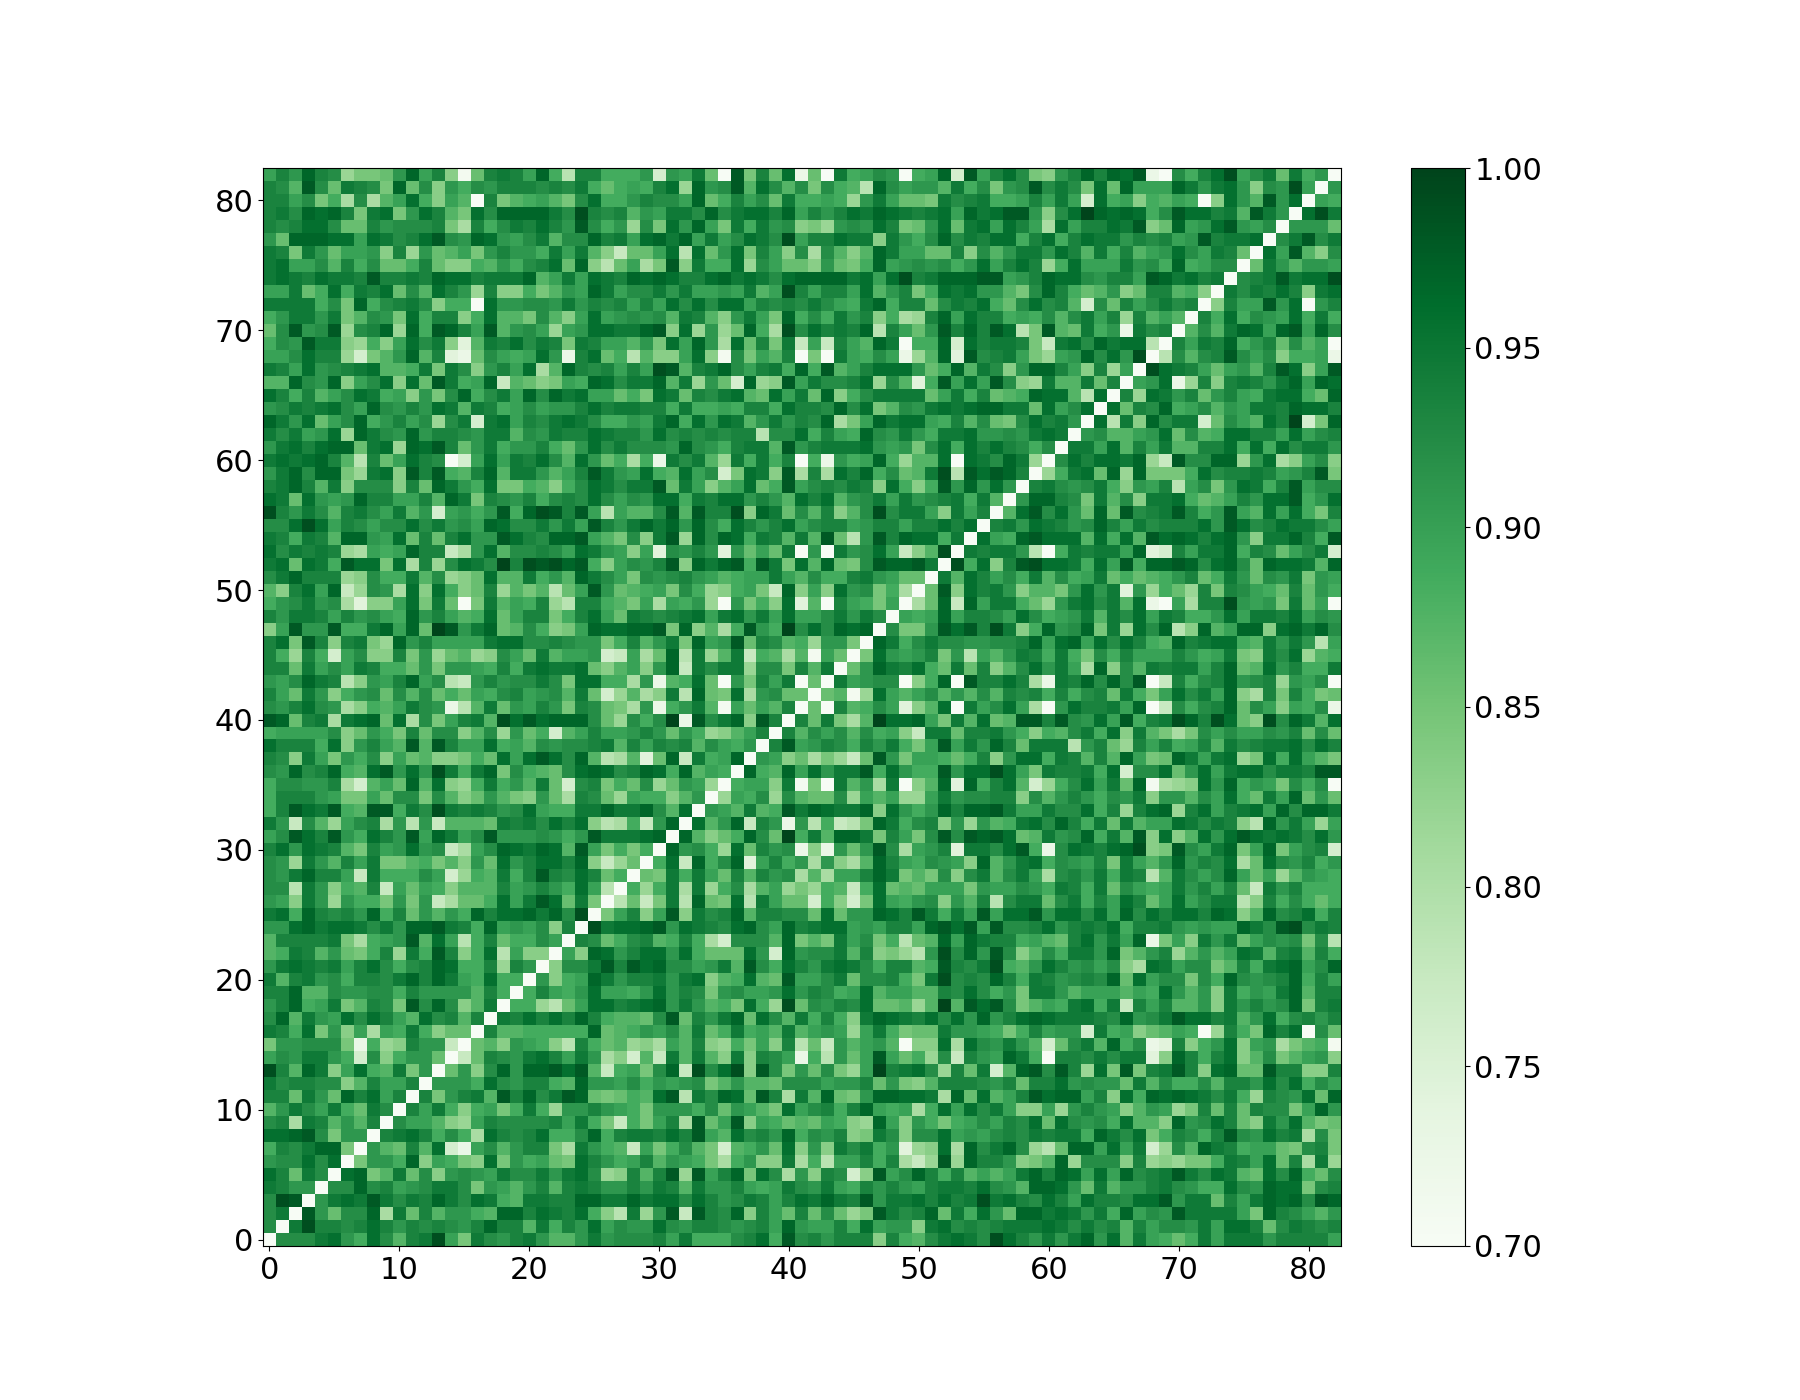
\includegraphics[width=\textwidth,height=12cm,keepaspectratio=true]{img/unigram_jaccard_50_green_07.png}
	\caption{
		Distanz zwischen den top 50 Unigrammen der Themen
	}
	\label{fig:Distanz_Unigramme}
\end{figure}

\begin{figure}[htpb]
	\centering
	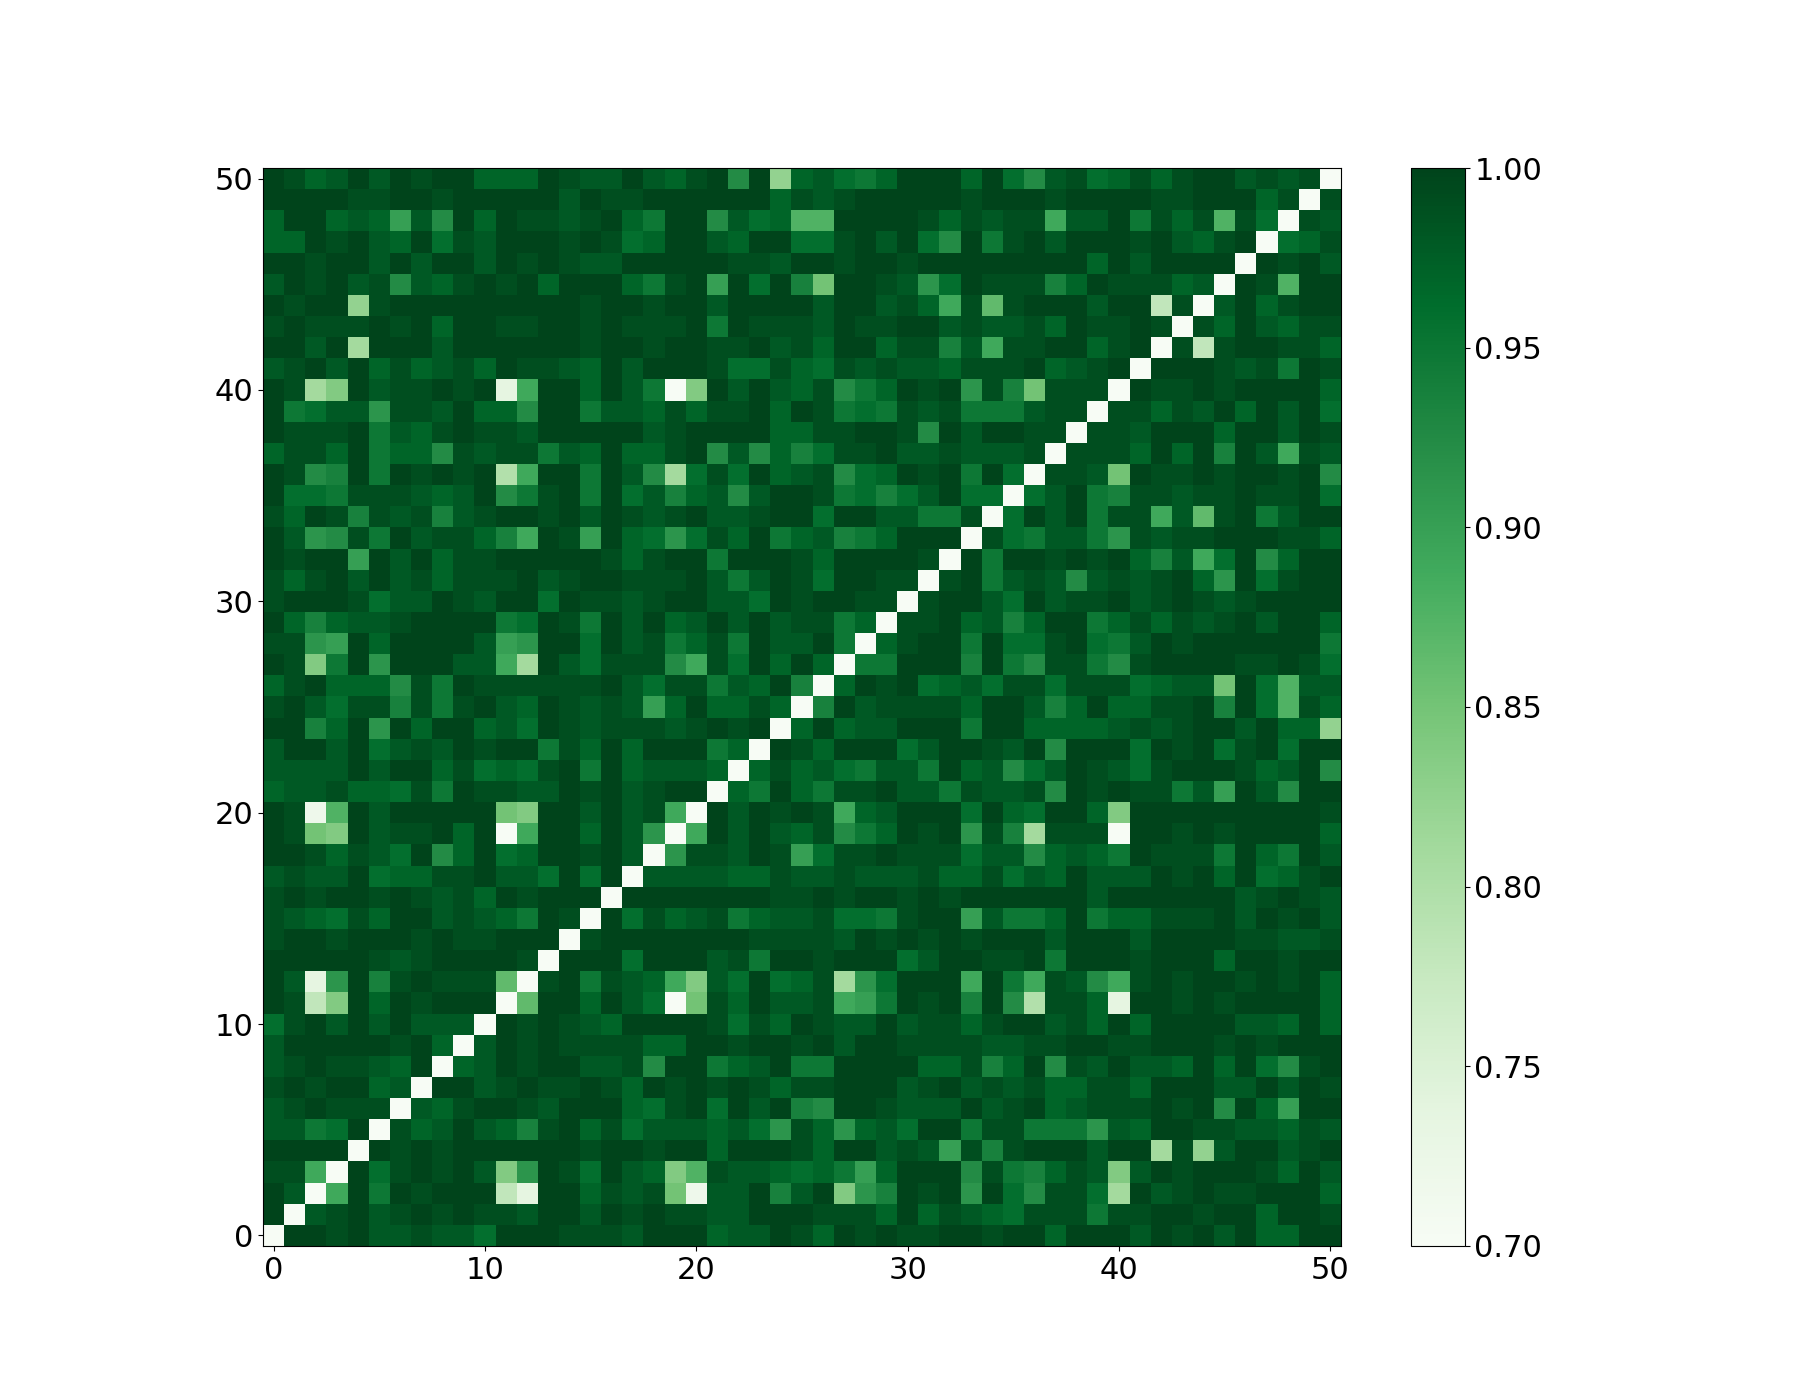
\includegraphics[width=\textwidth,height=12cm,keepaspectratio=true]{img/bigram_jaccard_50_green_07.png}
	\caption{
		Distanz zwischen den top 50 Bigrammen der Themen
	}
	\label{fig:Distanz_Bigramme}
\end{figure}


\section{Themengruppen}


\begin{figure}[htpb]
	\centering
	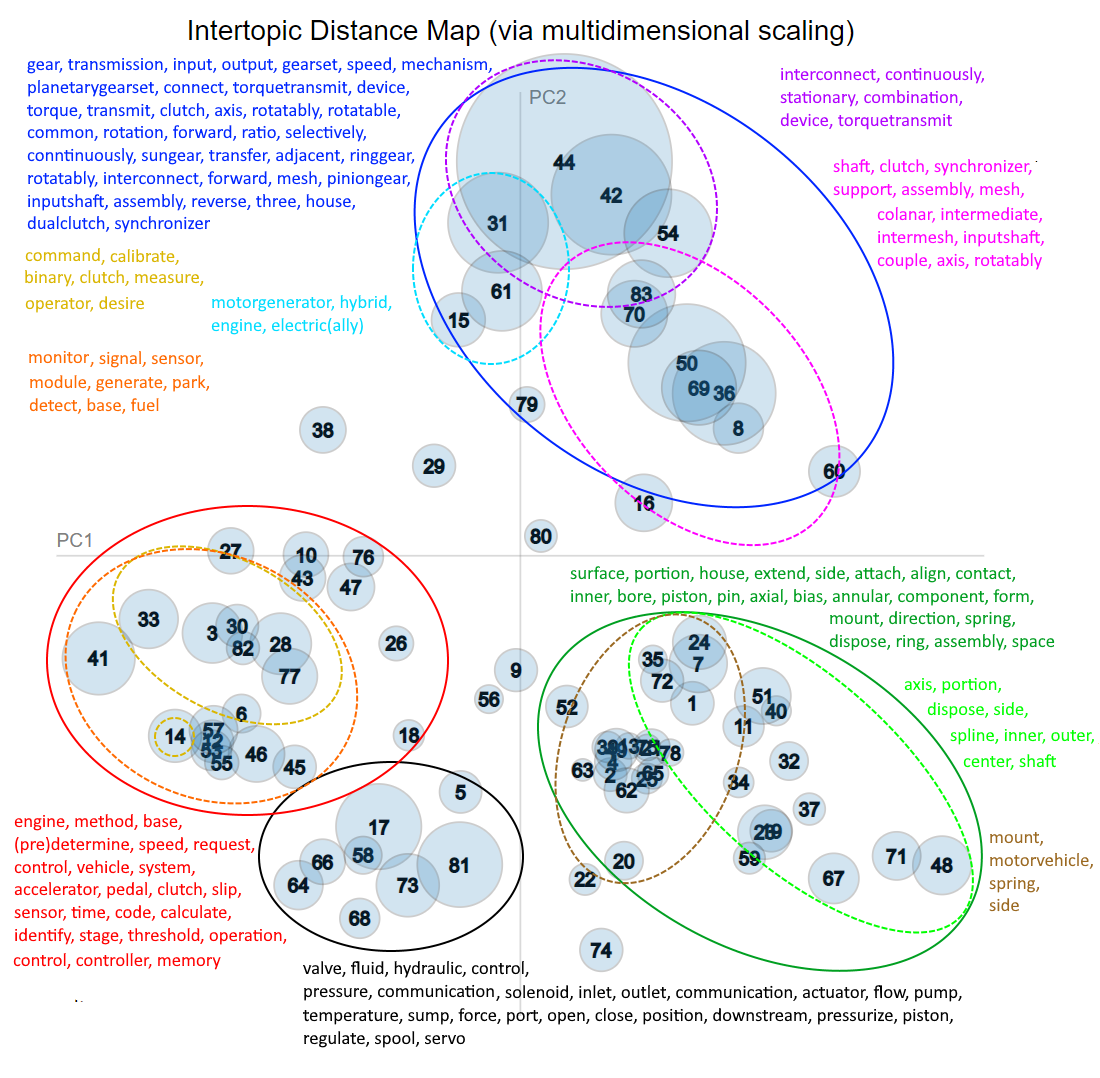
\includegraphics[width=\textwidth,height=10cm,keepaspectratio=true]{img/LDAvisGM-3-1-1clustered.png}
	\caption{
		Themengruppen der LDA Unigramme
	}
	\label{fig:Themengruppen_LDA_Unigramm}
\end{figure}


\section{Interpretation der Themen}

\begin{figure}[htpb]
	\centering
	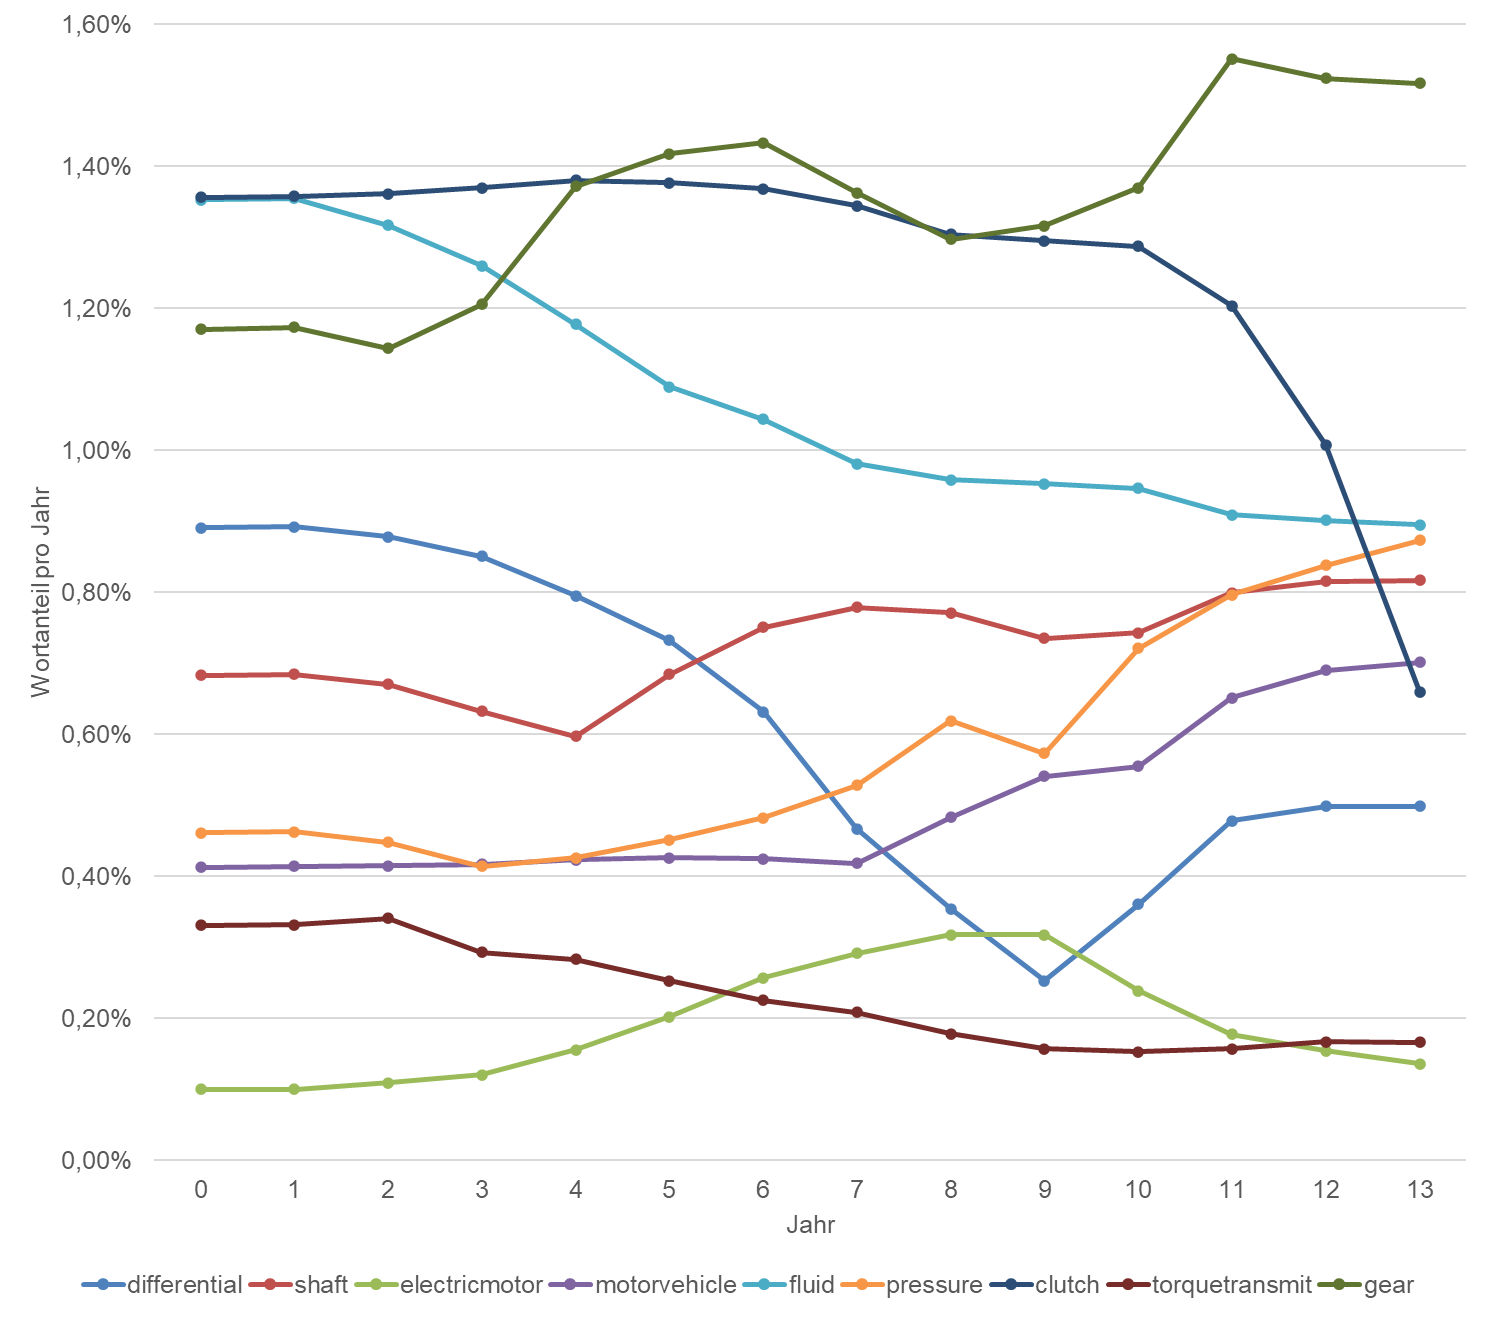
\includegraphics[width=\textwidth,height=12cm,keepaspectratio=true]{img/DLDA_unigram_01.png}
	\caption{
		Verlauf der Termhäufigkeit
	}
	\label{fig:DLDA_Unigramme_01}
\end{figure}